\subsection{Face Recognition System Implementation}

Before we can achieve our objective, we need a face recognition system to use as an attacking target. To recognise faces, we employ a pre-trained ResNet-18 model in pytorch.
In the neuron network, we use cross entropy loss as the loss function and stochastic gradient descent (SGD), a simple yet highly effective method for fitting linear classifiers and regressors under convex loss functions, as the optimizer. The model is trained for 10 iterations on the CelebA-HQ dataset.

\subsection{PGD Attack Modelling}

To generate adversarial examples, we use the PGD attack \cite{madry2017towards}. In this project, we use the gradient of the loss function to generate adversarial examples. The attack is iterative and uses a step size to determine the size of the perturbation. The attack is also constrained by a maximum perturbation size.

\subsubsection{Non-targeted Attack}

In a non-targeted attack, the goal is to generate an adversarial example that is misclassified by the target model $A$. Which means we are \textbf{maximizing} the loss function with respect to the target class $A$. The attack is as follows:

\begin{enumerate}
    \item Generate a random noise tensor $\delta$ with the same shape as the input image.
    \item Calculate the gradient of the loss function with respect to the noise tensor $\delta$.
    \item Add the gradient to the noise tensor $\delta$.
    \item Clip the noise tensor $\delta$ to the range $[-\epsilon, \epsilon]$.
    \item Add the noise tensor $\delta$ to the input image.
    \item Repeat steps 2 to 5 until the model misclassifies the image.
\end{enumerate}

The loss function (maximizing the difference with the true label) can be represented as:

\begin{center}
    \verb|Difference(Model(Face Image + Delta), True Label)|
\end{center}

where \verb|Model(Face Image + Delta)| is the prediction of perturbed data.


\begin{figure}[htbp]
    \centering
    \begin{subfigure}{0.4\textwidth}
        \centering
        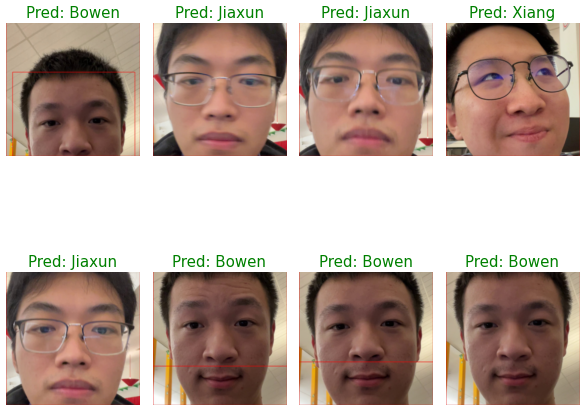
\includegraphics[width=1\textwidth]{pred_orig.png}
        \caption{Prediction without attack}
    \end{subfigure}
    \qquad
    \begin{subfigure}{0.4\textwidth}
        \centering
        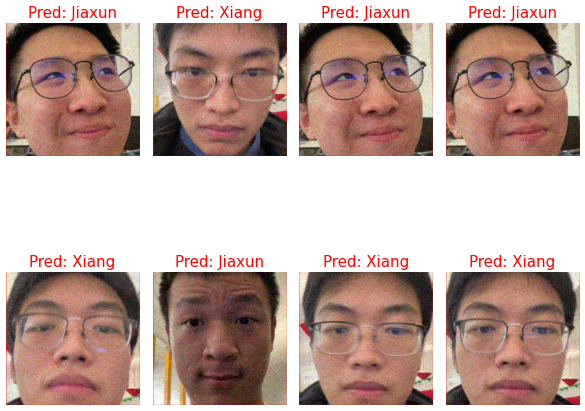
\includegraphics[width=1\textwidth]{pred_pgd_n.png}
        \caption{Prediction with non-targeted attack}
    \end{subfigure}
    \caption{Example of a non-targeted attack}
    \label{fig:pdf_attack_example}
\end{figure}

With above steps, we can generate an adversarial example that is misclassified by the target model. In figure \ref{fig:pdf_attack_example}, the image on the left demonstrates that Resnet-18 correctly predicted the original photos. After adding the PGD model's generated noise. The image on the right depicts Resnet-18 classifying the adversarial example as a different category.

\subsubsection{Targeted Attack}

In a targeted attack, the goal is to generate an adversarial example that is misclassified $A$ by the target model and classified as a specific class $B$. All the steps are the same as in a non-targeted attack, except for the last step should be: \textbf{Repeat steps 2 to 5 until the model classifies it as the target class.} Which means we are \textbf{minimizing} the loss function with respect to the target class $B$.

The loss function (minimizing the difference with the target label) can be represented as:

\begin{center}
    \verb|Difference(Model(Face Image + Delta), Target Label)|
\end{center}
